\documentclass[12pt, a4paper, UTF8]{ctexart}
\usepackage{geometry}
\usepackage{graphicx}
\usepackage{booktabs}
\usepackage{xcolor}
\usepackage{float}
\usepackage[hidelinks]{hyperref}
\usepackage{array}
\usepackage{multirow}
\usepackage{caption}
\usepackage{subcaption}

% 页面设置
\geometry{left=2.5cm, right=2.5cm, top=2.5cm, bottom=2.5cm}

% 标题设置
\ctexset{
    section={
        format=\Large\bfseries\centering,
        beforeskip=2ex plus 1ex minus 0.2ex,
        afterskip=2ex plus 0.2ex
    },
    subsection={
        format=\large\bfseries,
        beforeskip=1.5ex plus 1ex minus 0.2ex,
        afterskip=1.5ex plus 0.2ex
    },
    subsubsection={
        format=\normalsize\bfseries,
        beforeskip=1ex plus 0.5ex minus 0.2ex,
        afterskip=1ex plus 0.2ex
    }
}

\title{\heiti\zihao{2}制造系统建模与仿真实验报告}
\author{\kaishu\zihao{4}姓名：\underline{\qquad\qquad} \quad 学号：\underline{\qquad\qquad}}
\date{\kaishu\zihao{4}\today}

\begin{document}

% 封面
\begin{titlepage}
    \centering
    \vspace*{2cm}
    {\heiti\zihao{1}\textbf{制造系统建模与仿真}\\[0.5cm]
    \zihao{1}\textbf{实验报告}}\\[2cm]
    {\kaishu\zihao{3}\textbf{实验一：Witness 基本练习实验}}\\[3cm]
    {\songti\zihao{4}
    姓名：\underline{\qquad\qquad\qquad} \quad
    学号：\underline{\qquad\qquad\qquad} \quad
    班级：\underline{\qquad\qquad\qquad}\\[1.5cm]
    实验日期：\underline{\qquad\qquad\qquad} \quad
    报告日期：\underline{\qquad\qquad\qquad}
    }
    \vfill
\end{titlepage}

% 第一章：实验目的
\section{实验目的}
\begin{enumerate}
    \item 熟悉 Witness 仿真软件的界面布局和基本建模元素；
    \item 掌握使用 Witness 进行离散事件系统建模和仿真的基本流程；
    \item 熟悉 Witness 统计报表的生成方法，能够对仿真结果进行初步分析。
\end{enumerate}

% 第二章：实验内容
\section{实验内容}
本实验使用 Witness 仿真软件自带的 Stage4.mod 模型进行仿真练习。该模型模拟了一个简单的制造系统：小零件（widget）依次经过生产（Produce）、清洗（Wash）和称重（Weight）三道工序，每道工序前均设有缓冲区（Buffer）。零件清洗完成后通过传送带（Conveyor）运送至包装处（pack）。系统中有一名技术员（technician）负责完成所有作业，清洗机（wash machine）需要定时停机维修，防止故障发生时维修。

% 第三章：实验步骤
\section{实验步骤}
\begin{enumerate}
    \item 启动 Witness 仿真系统；
    \item 熟悉 Witness 仿真系统的菜单栏、工具栏和各类对话框；
    \item 打开仿真项目 Stage4.mod；
    \item 设置仿真运行时间为 1440 min（24 h），运行仿真项目；
    \item 仿真结束后，生成 Part Statistics 等统计报表，观察并记录仿真结果；
    \item 根据仿真数据整理并填写实验报告。
\end{enumerate}

% 第四章：仿真模型说明
\section{仿真模型说明}
Stage4.mod 模型的逻辑结构如图 \ref{fig:model} 所示。该模型中包含以下建模元素：

\begin{table}[H]
    \centering
    \caption{Stage4.mod 模型建模元素}
    \label{tab:elements}
    \small
    \begin{tabular}{clll}
        \toprule
        \textbf{元素类型} & \textbf{元素名称} & \textbf{功能说明} \\
        \midrule
        Part & widget & 待加工的小零件 \\
        Machine & produce & 生产工序 \\
        Buffer & Qwash & 清洗前等待队列 \\
        Machine & Wash & 清洗工序 \\
        Buffer & Qweigh & 称重前等待队列 \\
        Machine & Mc\_Weigh001 & 称重工序 \\
        Conveyor & Conveyor001 & 传送带，运输零件 \\
        Labor & technician & 技术员，负责操作 \\
        Machine & pack & 包装工序 \\
        Variable & numbershipped & 出货数量统计变量 \\
        \bottomrule
    \end{tabular}
\end{table}

模型工艺流程为：widget 零件从 produce 工序进入系统，经 Qwash 缓冲后进入 Wash 清洗，清洗后经 Qweigh 缓冲进入 Mc\_Weigh001 称重，随后通过 Conveyor001 传送带运送至 pack 包装，最终完成出货（SHIP）。technician 作为共享资源，在各工序间调度作业。Wash 工序设置了定时维修机制，以模拟设备预防性维护。

\begin{figure}[H]
    \centering
    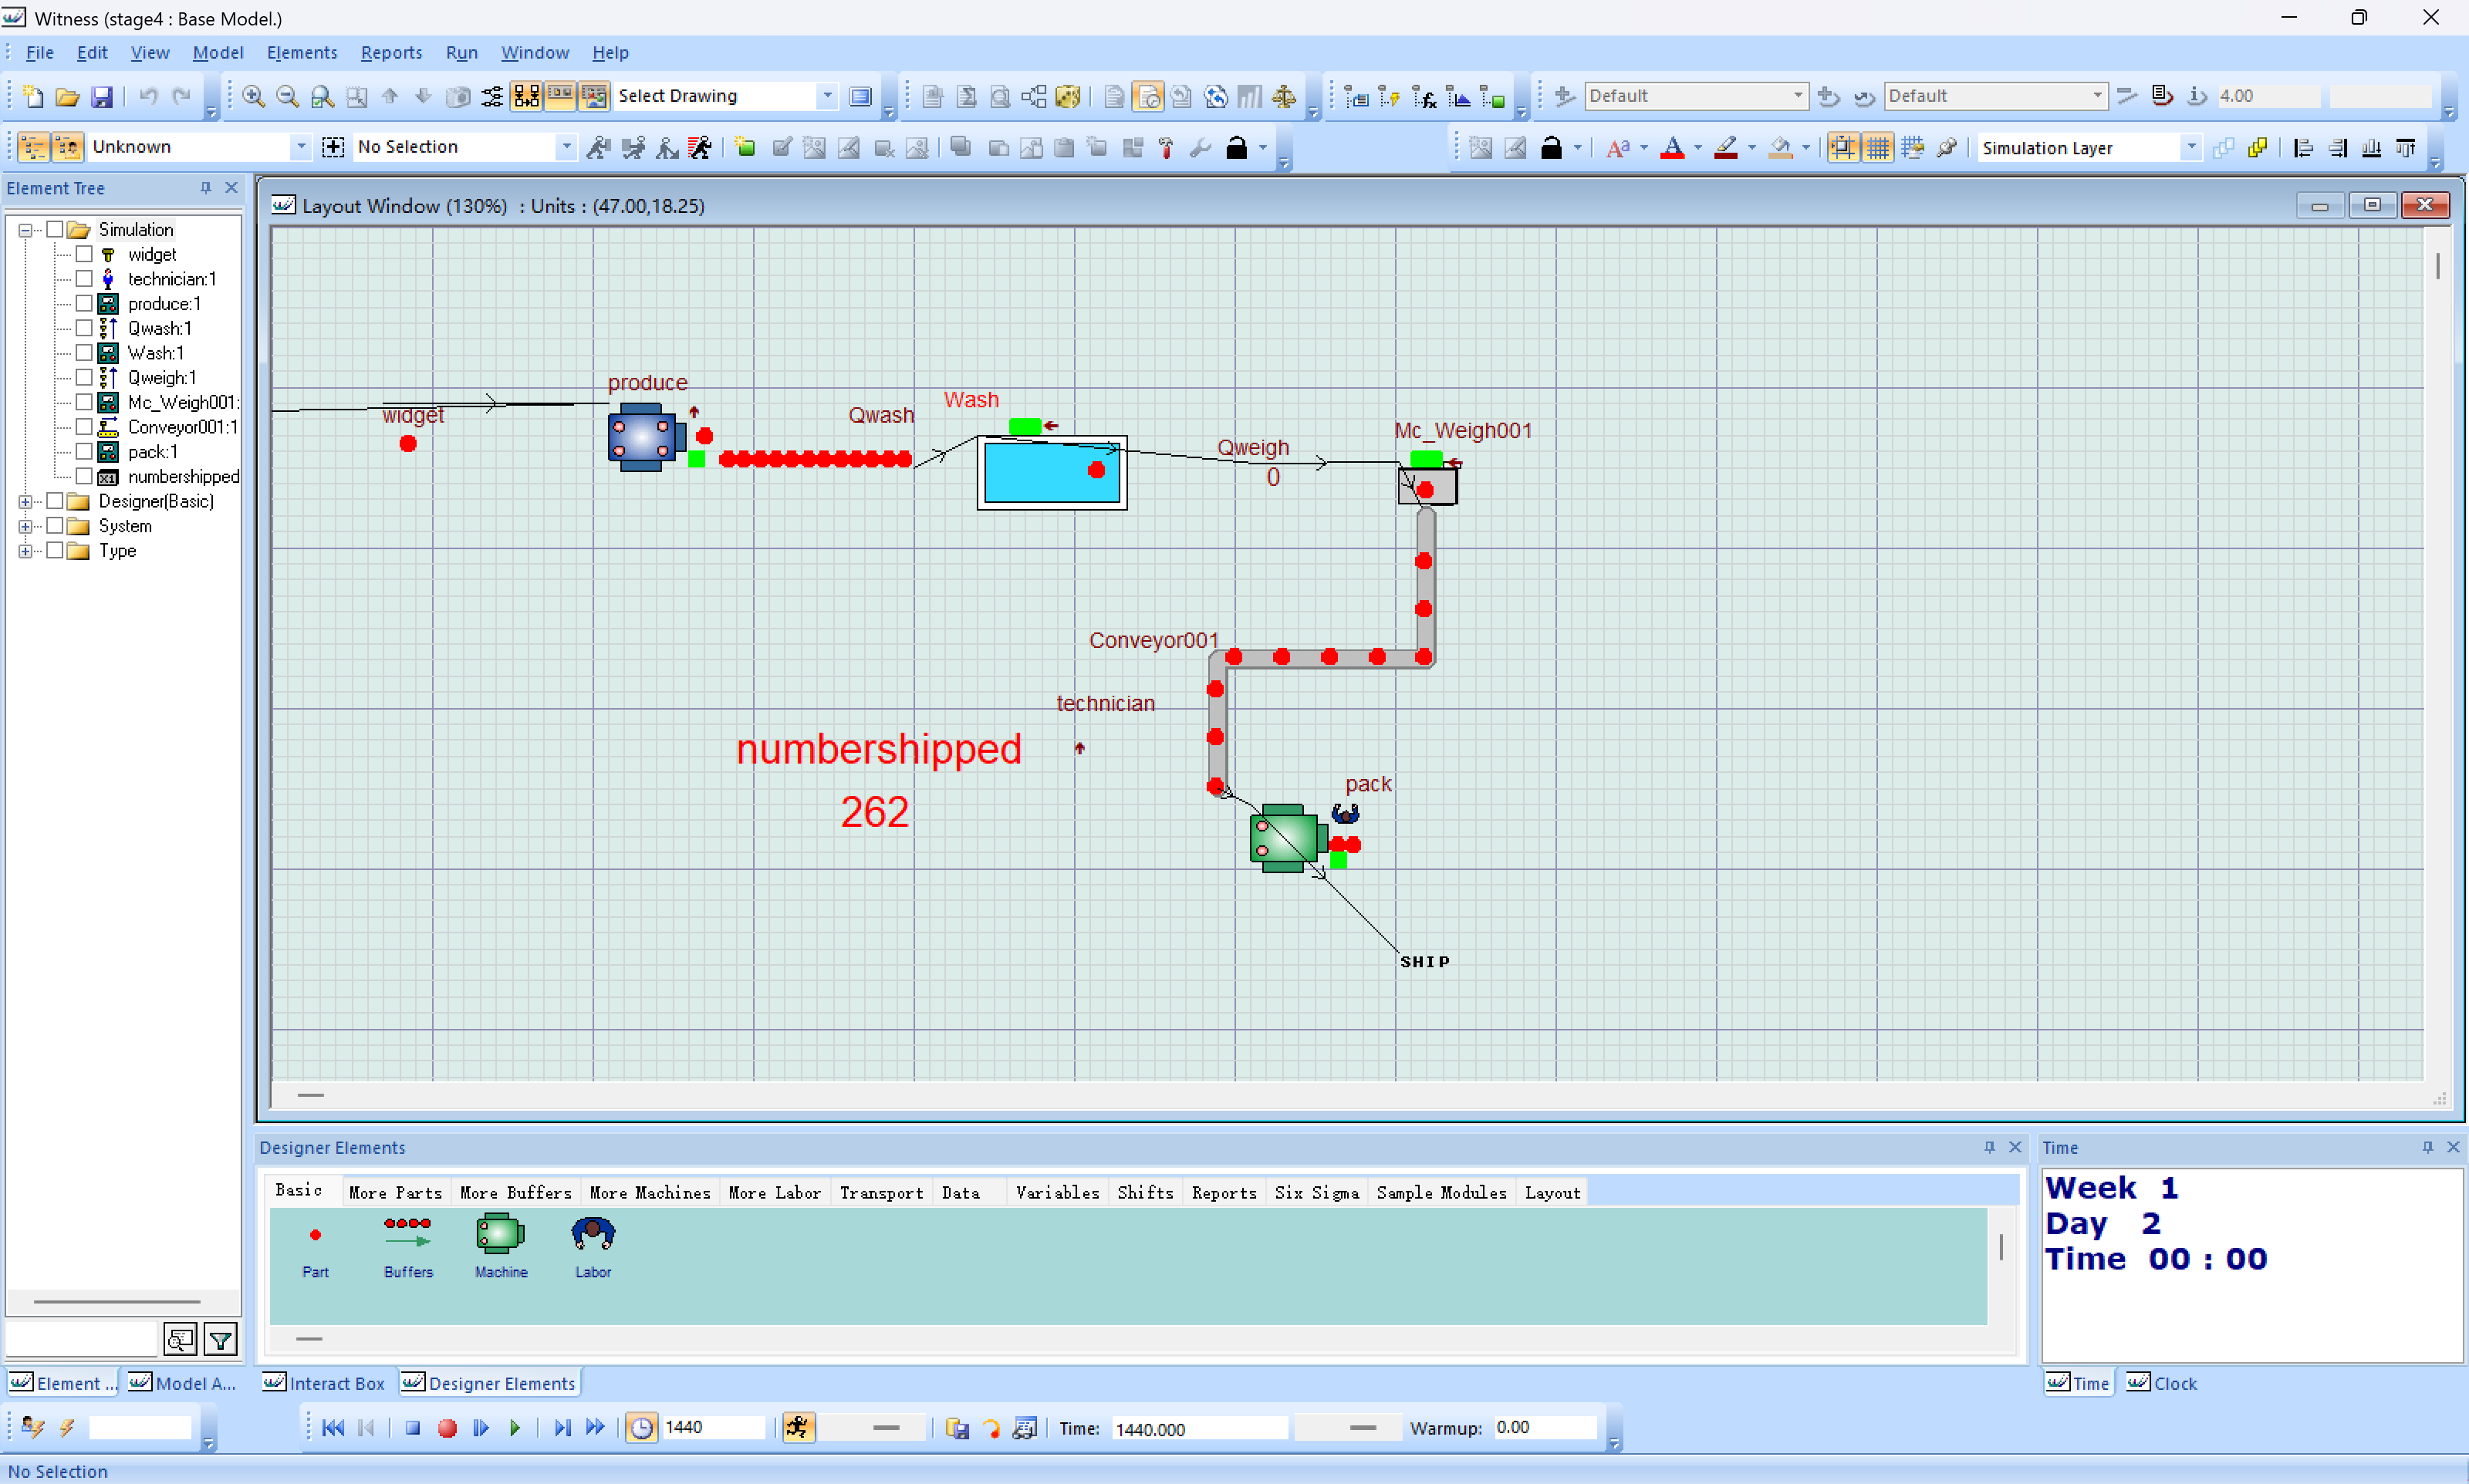
\includegraphics[width=0.75\textwidth]{../实验一_模型截图.png}
    \caption{Stage4.mod 仿真模型截图}
    \label{fig:model}
\end{figure}

% 第五章：仿真结果分析
\section{仿真结果分析}
仿真运行 1440 min 后，生成各类统计报表。下文分别对 Part、Machine、Buffer、Conveyor、Labor 和 Variable 的统计结果进行分析。

\smallskip
\noindent\textbf{报表术语说明}：No. Entered（进入数量）、No. Shipped（出货数量）、No. Scrapped（报废数量）、No. Rejected（拒收数量）、W.I.P.（当前在制品）、Avg W.I.P.（平均在制品数）、Avg Time（平均通过时间）、Sigma Rating（西格玛等级）、\% Idle（空闲率）、\% Busy（忙碌率）、\% Broken Down（故障率）、\% Setup（设置率）、\% Cycle Wait（循环等待率）、No. Of Operations（操作次数）、Total In/Out（进入/离开数量）、Now In（当前数量）、Avg Size（平均大小）、\% Empty/Move/Blocked/Queue（传送带空/移动/阻塞/排队率）、\% Busy/Idle（劳动力忙碌/空闲率）、No. Of Jobs（作业次数）、Avg Job Time（平均作业时间）。下文不再重复标注。

\subsection{Part Statistics}
widget 零件的 Part Statistics 统计结果如表 \ref{tab:part_stats} 所示，原始报表截图见图 \ref{fig:part_stats}。

\begin{table}[H]
    \centering
    \caption{widget 零件 Part Statistics 统计结果}
    \label{tab:part_stats}
    \begin{tabular}{lc}
        \toprule
        \textbf{统计指标} & \textbf{数值} \\
        \midrule
        No. Entered & 289 \\
        No. Shipped & 262 \\
        No. Scrapped & 0 \\
        No. Assembled & 0 \\
        No. Rejected & 0 \\
        W.I.P. & 27 \\
        Avg W.I.P. & 24.46 \\
        Avg Time & 121.89 min \\
        Sigma Rating & 6.00 \\
        \bottomrule
    \end{tabular}
\end{table}

在 1440 min 的仿真周期内，共有 289 个零件进入系统，其中 262 个成功出货，当前系统内有 27 个在制品。零件的平均通过时间为 121.89 min，系统无报废和拒收零件，西格玛等级为 6.00，说明系统整体质量水平较高。

\begin{figure}[H]
    \centering
    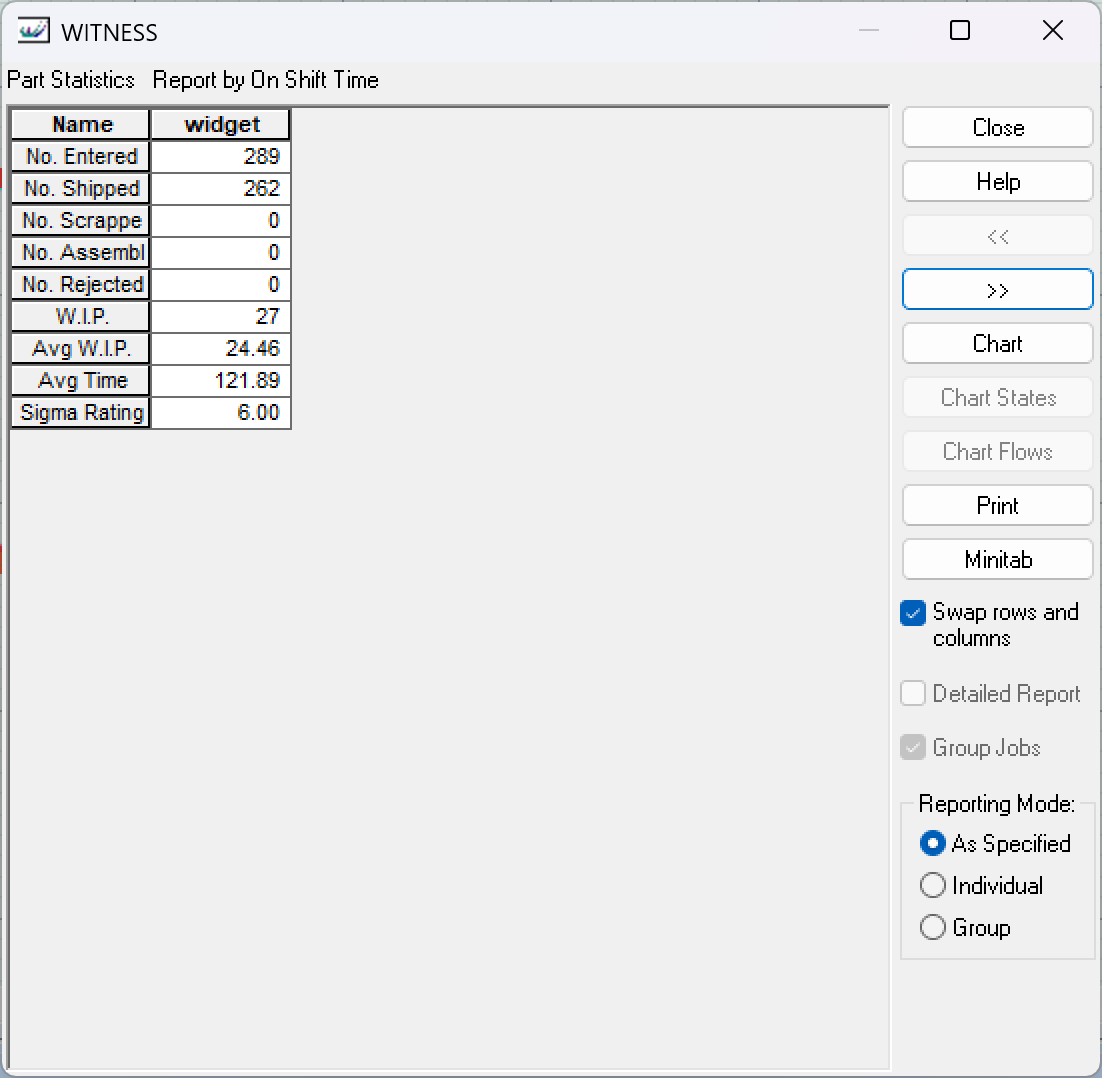
\includegraphics[width=0.75\textwidth]{../实验一_Part_Statistics.png}
    \caption{Part Statistics 运行结果截图}
    \label{fig:part_stats}
\end{figure}

\subsection{Machine Statistics}
四台机器的 Machine Statistics 统计结果如表 \ref{tab:machine_stats} 所示，原始报表截图见图 \ref{fig:machine_stats}。

\begin{table}[H]
    \centering
    \caption{Machine Statistics 统计结果}
    \label{tab:machine_stats}
    \small
    \begin{tabular}{lcccc}
        \toprule
        \textbf{统计指标} & \textbf{produce} & \textbf{Wash} & \textbf{Mc\_Weigh001} & \textbf{pack} \\
        \midrule
        \% Idle & 0.00 & 1.95 & 42.75 & 17.38 \\
        \% Busy & 100.00 & 76.56 & 57.25 & 63.96 \\
        \% Blocked & 0.00 & 0.00 & 0.00 & 0.00 \\
        \% Cycle Wait & 0.00 & 0.00 & 0.00 & 18.66 \\
        \% Setup & 0.00 & 1.26 & 0.00 & 0.00 \\
        \% Broken Down & 0.00 & 19.08 & 0.00 & 0.00 \\
        \% Repair Wait & 0.00 & 1.16 & 0.00 & 0.00 \\
        No. Of Operations & 288 & 275 & 274 & 131 \\
        \bottomrule
    \end{tabular}
\end{table}

从表中可以看出，produce 工序的忙碌率达到 100\%，说明该工序始终处于满负荷状态，是系统的入口环节。Wash 工序忙碌率为 76.56\%，但有 19.08\% 的时间处于故障停机状态，另有 1.26\% 的时间用于设置和 1.16\% 的维修等待时间，这与模型中设置的定时维修机制一致。Mc\_Weigh001 的空闲率高达 42.75\%，说明称重工序有较多的空闲等待时间。pack 工序有 18.66\% 的循环等待时间，表明包装工序有时需要等待上游零件到达。

\begin{figure}[H]
    \centering
    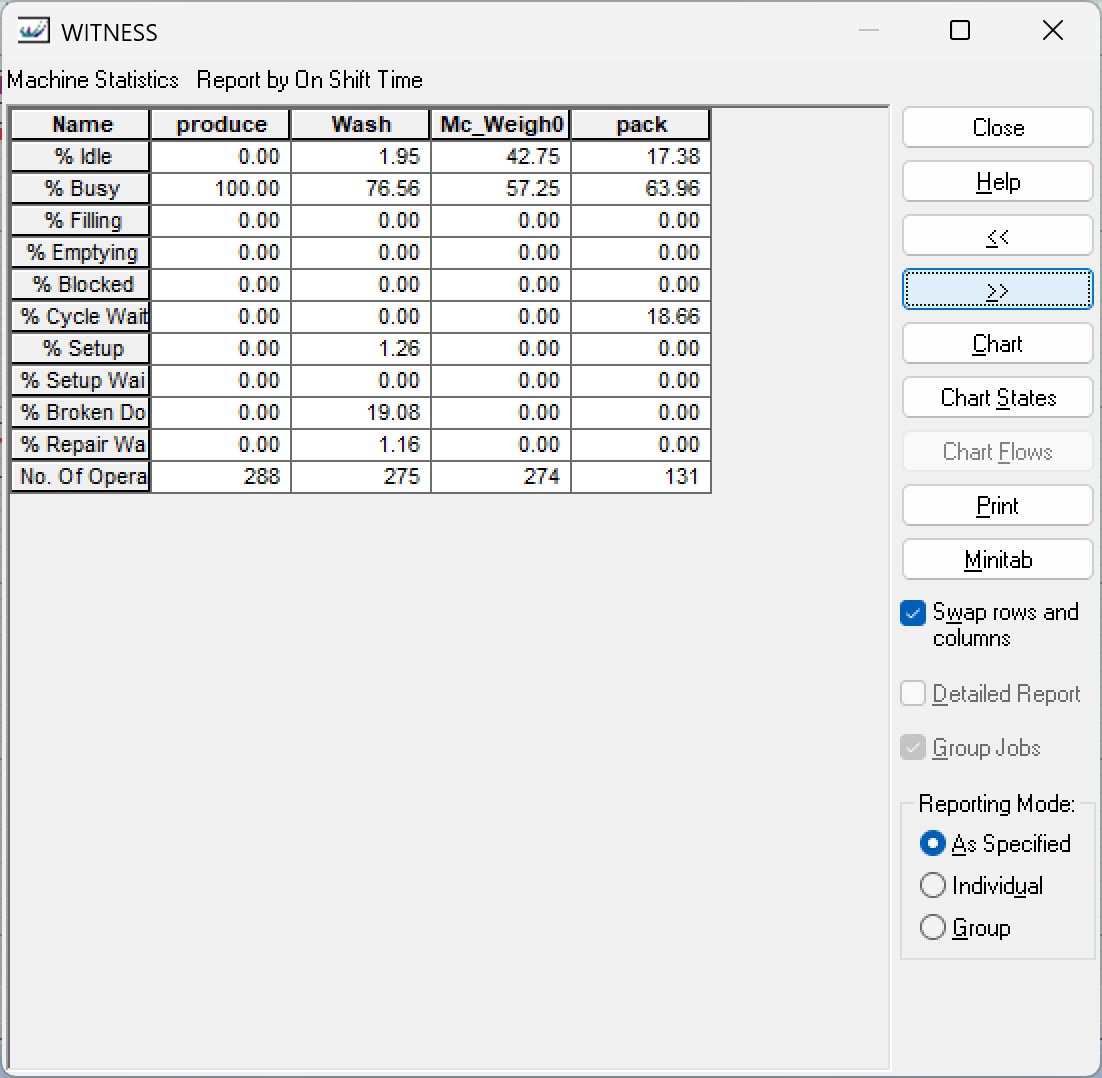
\includegraphics[width=0.75\textwidth]{../实验一_Machine_Statistics.png}
    \caption{Machine Statistics 运行结果截图}
    \label{fig:machine_stats}
\end{figure}

\subsection{Buffer Statistics}
两个缓冲区的 Buffer Statistics 统计结果如表 \ref{tab:buffer_stats} 所示，原始报表截图见图 \ref{fig:buffer_stats}。

\begin{table}[H]
    \centering
    \caption{Buffer Statistics 统计结果}
    \label{tab:buffer_stats}
    \begin{tabular}{lcc}
        \toprule
        \textbf{统计指标} & \textbf{Qwash} & \textbf{Qweigh} \\
        \midrule
        Total In & 288 & 275 \\
        Total Out & 276 & 275 \\
        Now In & 12 & 0 \\
        Max & 23 & 1 \\
        Min & 0 & 0 \\
        Avg Size & 11.09 & 0.00 \\
        Avg Time & 55.45 & 0.00 \\
        Min Time & 0.00 & 0.00 \\
        Max Time & 110.96 & 0.00 \\
        \bottomrule
    \end{tabular}
\end{table}

Qwash 缓冲区的平均大小为 11.09，最大值达到 23，说明清洗工序前有较多零件排队等待，这与 Wash 机器因故障和设置导致的停机时间有关。仿真结束时 Qwash 中仍有 12 个零件等待。Qweigh 缓冲区的各项指标几乎为零，说明称重工序前基本没有排队现象，零件到达后可以立即进入称重工序。

\begin{figure}[H]
    \centering
    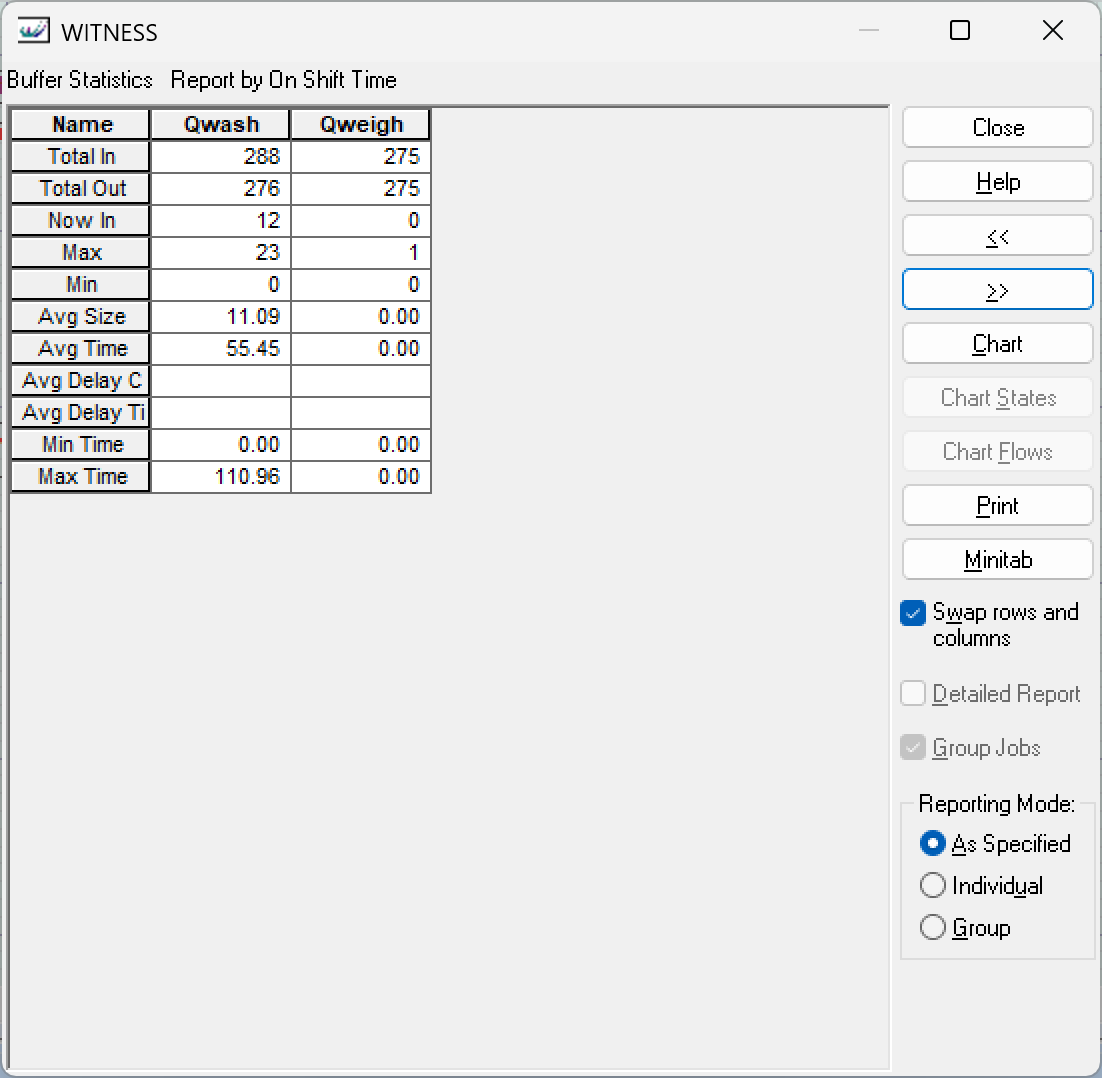
\includegraphics[width=0.75\textwidth]{../实验一_Buffer_Statistics.png}
    \caption{Buffer Statistics 运行结果截图}
    \label{fig:buffer_stats}
\end{figure}

\subsection{Conveyor Statistics}
传送带 Conveyor001 的统计结果如表 \ref{tab:conveyor_stats} 所示，原始报表截图见图 \ref{fig:conveyor_stats}。

\begin{table}[H]
    \centering
    \caption{Conveyor Statistics 统计结果}
    \label{tab:conveyor_stats}
    \begin{tabular}{lc}
        \toprule
        \textbf{统计指标} & \textbf{Conveyor001} \\
        \midrule
        \% Empty & 0.83 \\
        \% Move & 42.50 \\
        \% Blocked & 0.00 \\
        \% Queue & 56.67 \\
        \% Broken Down & 0.00 \\
        Now On & 10 \\
        Total On & 274 \\
        Avg Size & 9.04 \\
        Avg Time & 47.51 \\
        \bottomrule
    \end{tabular}
\end{table}

传送带的排队率高达 56.67\%，说明零件在传送带上等待的时间比例较大，这主要是因为下游包装工序的处理速度有限。传送带平均大小为 9.04，仿真结束时有 10 个零件在传送带上。传送带没有发生阻塞和故障，运行较为稳定。

\begin{figure}[H]
    \centering
    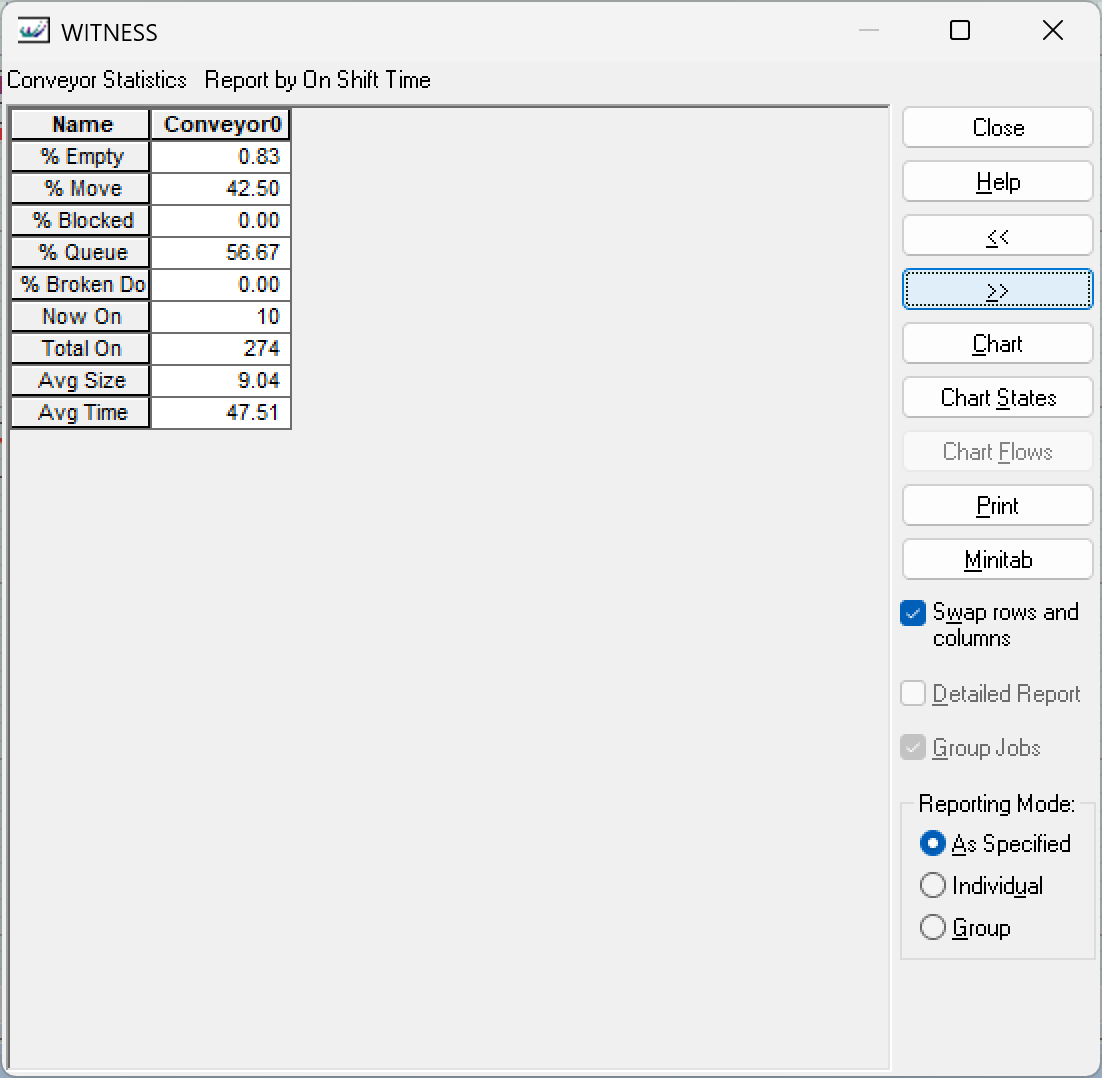
\includegraphics[width=0.75\textwidth]{../实验一_Conveyor_Statistics.png}
    \caption{Conveyor Statistics 运行结果截图}
    \label{fig:conveyor_stats}
\end{figure}

\subsection{Labor Statistics}
技术员 technician 的统计结果如表 \ref{tab:labor_stats} 所示，原始报表截图见图 \ref{fig:labor_stats}。

\begin{table}[H]
    \centering
    \caption{Labor Statistics 统计结果}
    \label{tab:labor_stats}
    \begin{tabular}{lc}
        \toprule
        \textbf{统计指标} & \textbf{technician} \\
        \midrule
        \% Busy & 83.04 \\
        \% Idle & 16.96 \\
        Quantity & 1 \\
        No. Of Jobs & 136 \\
        Avg Job Time & 8.83 \\
        \bottomrule
    \end{tabular}
\end{table}

技术员的忙碌率为 83.04\%，完成了 136 次作业，平均每次作业时间为 8.83 min。技术员在系统中承担了 Wash 工序的设置和维修操作，16.96\% 的空闲率说明技术员偶尔有等待时间，整体利用率较高。

\begin{figure}[H]
    \centering
    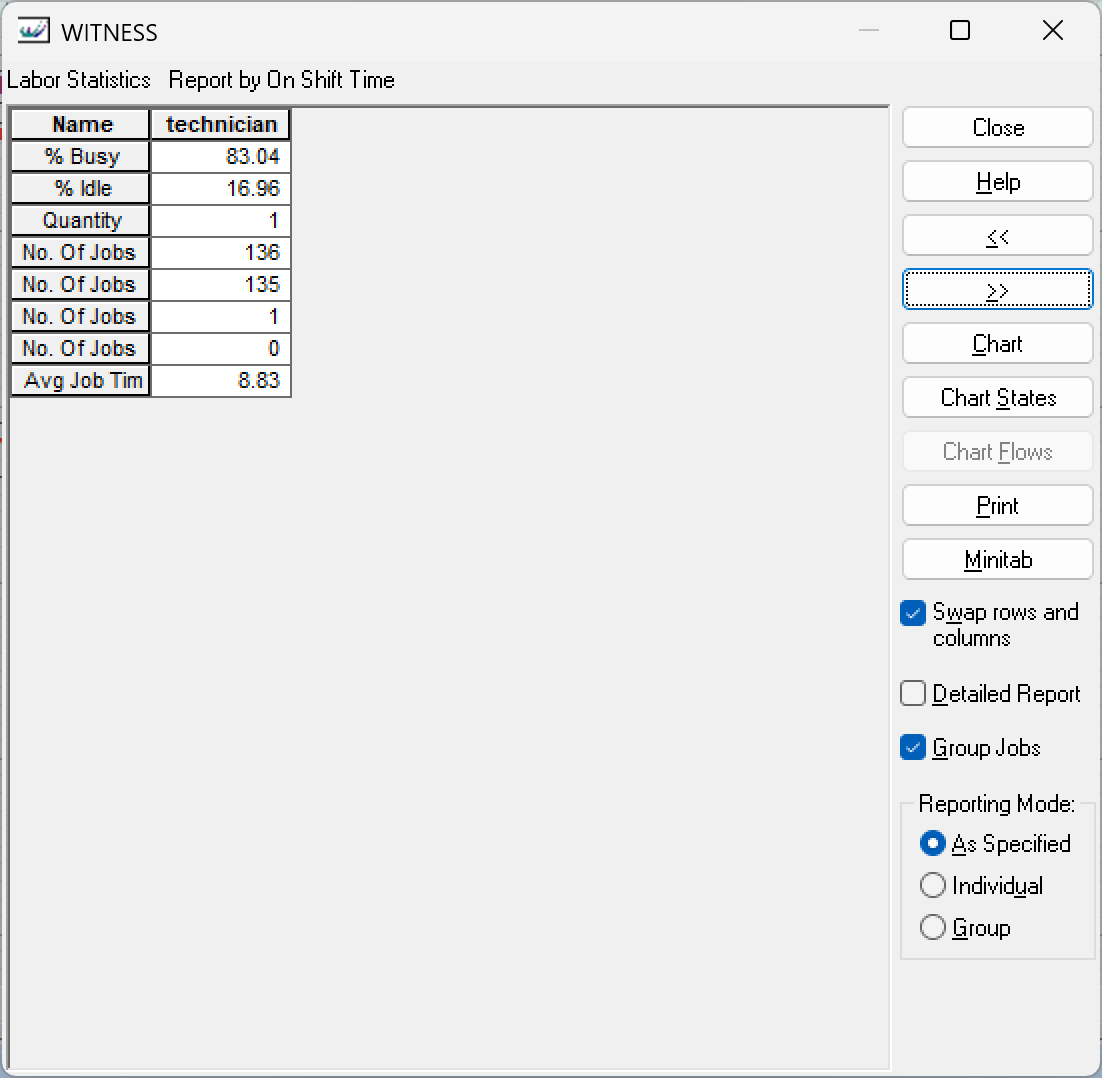
\includegraphics[width=0.75\textwidth]{../实验一_Labor_Statistics.png}
    \caption{Labor Statistics 运行结果截图}
    \label{fig:labor_stats}
\end{figure}

\subsection{Variable Statistics}
变量 numbershipped 用于统计出货数量，其值为 262，与 Part Statistics 中的 No. Shipped 一致，验证了仿真结果的正确性。原始报表截图见图 \ref{fig:variable_stats}。

\begin{figure}[H]
    \centering
    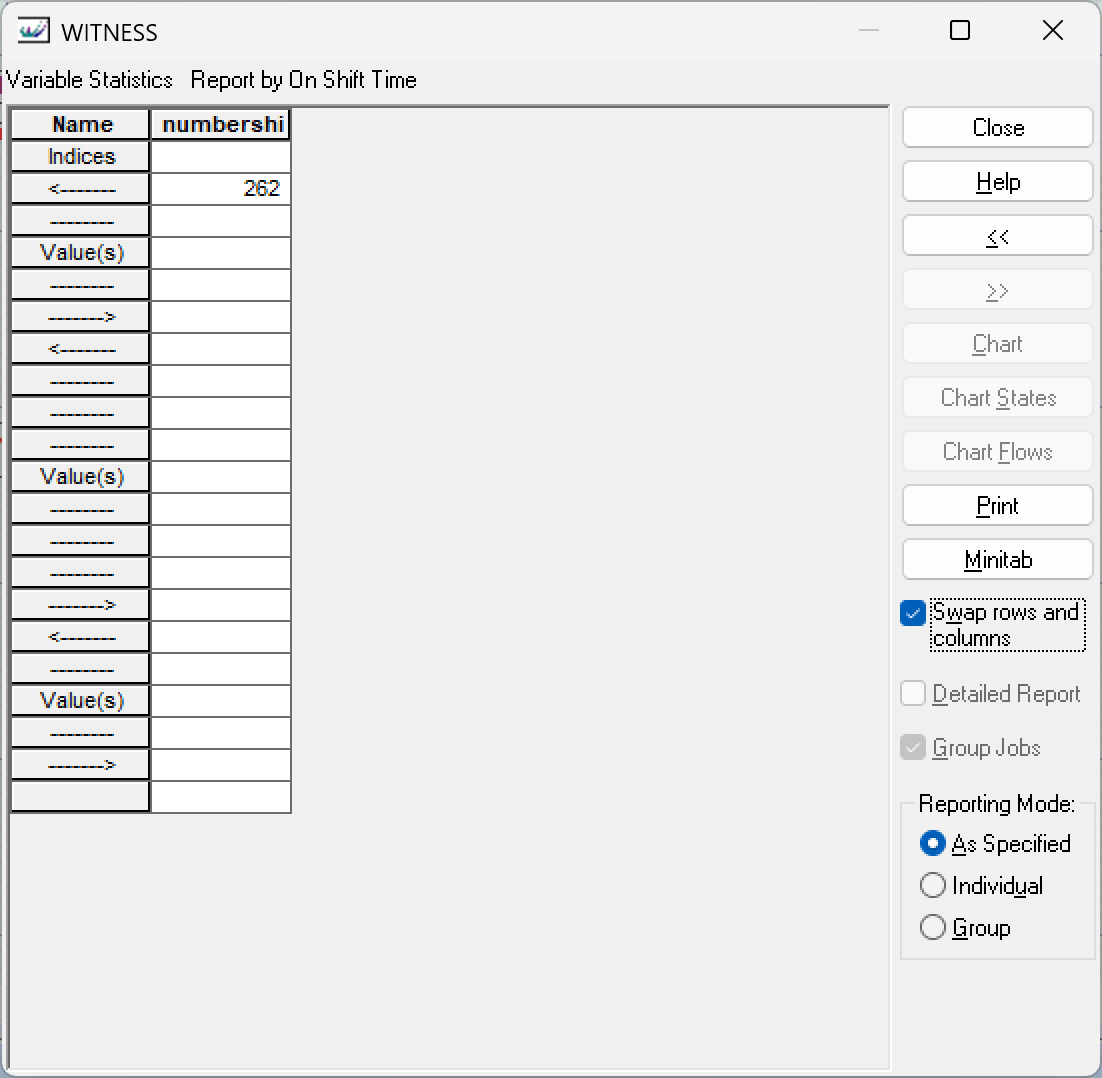
\includegraphics[width=0.75\textwidth]{../实验一_Variable_Statistics.png}
    \caption{Variable Statistics 运行结果截图}
    \label{fig:variable_stats}
\end{figure}

% 第六章：思考题
\section{思考题}

\subsection{Witness 系统的文件类型有哪些？}
Witness 系统的主要文件类型包括：.mod（模型文件，存储仿真模型的结构和逻辑）、.dat（数据文件，存储仿真数据）、.rep（报表文件，存储仿真结果报表）、.txt（文本文件，用于导入导出数据）等。

\subsection{Witness 系统菜单栏有哪些？}
Witness 系统菜单栏主要包括：File（文件）、Edit（编辑）、View（视图）、Model（模型）、Elements（元素）、Reports（报表）、Run（运行）、Window（窗口）、Help（帮助）等。

\subsection{Witness 系统中有哪些建模元素？}
Witness 系统提供了丰富的建模元素，主要包括：Part（零件）、Machine（机器/工序）、Buffer（缓冲区）、Conveyor（传送带）、Labor（劳动力/人员）、Vehicle（车辆）、Track（轨道）、Path（路径）、Variable（变量）、Attribute（属性）、Timeseries（时间序列）等。这些元素分为物理元素和逻辑元素两大类。

\subsection{Stage4.mod 仿真项目中用到了哪些建模元素？}
Stage4.mod 项目中用到的建模元素包括：Part（widget）、Machine（produce、Wash、Mc\_Weigh001、pack）、Buffer（Qwash、Qweigh）、Conveyor（Conveyor001）、Labor（technician）、Variable（numbershipped）等。

% 第七章：实验心得体会
\section{实验心得体会}
\begin{enumerate}
    \item 通过本次实验，我对 Witness 仿真软件有了初步的认识。Witness 采用面向对象的建模思想，通过拖拽不同的建模元素并设置其属性，可以快速构建离散事件系统仿真模型。
    \item 我学会了如何打开已有模型、设置仿真运行时间、启动仿真以及查看和解读统计报表，这些都是后续实验的基础。
    \item Stage4.mod 模型虽然结构相对简单，但涵盖了零件、机器、缓冲区、传送带、人员等多种典型的制造系统要素，较好地展示了一个基本生产线的运行逻辑。
    \item 从仿真结果来看，该系统在 1440 min 的运行周期内完成了 262 个零件的加工和出货，平均通过时间约 122 min，系统运行较为平稳。
    \item 仿真技术是分析和优化制造系统的重要工具，通过建立仿真模型，可以在不干扰实际生产的情况下观察系统运行状态、识别瓶颈环节、评估不同方案的效果，为生产决策提供科学依据。
\end{enumerate}

\end{document}
